\chapter{Hull-White Single-Factor Model}
\label{chapter:hullwhitemodel}

\subsection{Overview}
Pricing a single option using Hull-White single-factor trinomial tree model consists of two steps. The first (forward propagation along the tree) is the construction of the trinomial tree in order to obtain a list of alpha values for each time step. These alphas are later used in the second step (backward propagation along the tree) to fit the option/bond prices and obtain the option value back at the root node of the tree. The input fed to the algorithm consists of a list of options, as for each option the information provided is its strike price, maturity, time step length, reversion rate\footnote{denoted as $a$ - determines the relative volatilities of long and short rates\cite[pg.9]{npfits}} and volatility\footnote{denoted as $\sigma$ - determines the overall level of volatility \cite[pg. 9]{npfits}}. The output is a list of option values for each inputted option/bond. The two steps can be generalized as follows: 

\begin{enumerate}
    \item \textbf{Forward propagation step:} Construct a term structure for the underlying asset by progressing one time step at a time. Determine neutral risk rate for a new time step using estimated yield curve data and estimated current asset values.
    \item \textbf{Backward propagation step:} Discount the asset prices to estimate option payoff at maturity going from the leaves of the tree to its root. 
\end{enumerate}

Algorithm~\ref{alg:loops} shows a high-level overview of a function implementing this procedure for pricing of one option. The function mainly consists of two sequential (convergence) loops of count N, which contain inner parallel operators of length M, where N and M are specific to each option (and thus vary across options). M corresponds to the tree width which is dependent on the number of terms and input parameters. N corresponds to the tree height which is dependent on the number of time steps (maturity of the underlying bond and precision).

\begin{algorithm}[H]
    \DontPrintSemicolon
    \caption{High-level overview of pricing a single option using Hull-White 1F model     \label{alg:loops}}
    \SetKwFunction{Range}{range}
    
    \tcc{forward propagation (convergence) loop}
    \For{$i := 0$ \KwTo $N$} {
        \For{$j := 0$ \KwTo $M$} {
            write\;
        }
        reduce\;
    }
    
    \tcc{backward propagation (convergence) loop}
    \For{$i := N$ \KwTo $0$} {
        \For{$j := 0$ \KwTo $M$} {
            write\;
        }
    }
\end{algorithm}

Different option/bond maturities (leading to different tree widths) and different level of pricing accuracy (number of simulated time steps leading to different tree heights) make choosing an effective parallelization strategy difficult and in order to achieve maximum parallelization efficiency, it is necessary to have a deep understanding of the algorithm itself. The book by John Hull\cite{ofod} provides a solid background on the topic, describing the mechanics of interest rates, markets, the need for binomial trees and how that has led to the use of trinomial trees. Chapter 30 further narrows the topic of using trinomial trees as a numerical method and introduces a step by step walk-through of applying the algorithm on a basic example. While some of the calculation details are omitted in the book, the authors provide references to previous articles\cite{npfits}\cite{uhwirt}, where they explain them. 

% TODO: trinomial tree is discrete-time; lattice based???
It is important to mention that the construction of a trinomial tree is a discrete-time, lattice-based\footnote{A model that takes into account expected changes in various parameters e.g. volatility over the duration of the options} numerical method, but the example in the book is simplified by cutting the tree at a certain height and using analytic formulas to produce a concrete result for a specific financial instrument - a zero-coupon bond maturing at time $(m + 1) * \triangle t$ \cite[pg. 704]{ofod}. These formulas have been found and proven to be effective by the authors of the book and the articles. While this simplification gives more precise results in the above mentioned specific case, constructing the entire tree and using all of the time steps can also give a good approximation for other financial instruments, even though being computationally intensive. All the implementations of this thesis will be focused on the numerical approach.

The following sub-chapters are focused primarily on the intuition behind the algorithm, with the sole purpose to provide the reader with a general overview for it. For this reason, many of the details and formulas of calculating specific values have been omitted, however they are thoroughly described in the book and the articles by Hull and White. As the model is best understood visually, we have included some of the supplementary images from the Hull and White book in order to support our algorithm explanation. 

\subsection{Forward propagation}
The forward propagation by itself consists of two stages. Each of them computes different values on the same tree. While the tree height can grow indefinitely, depending on the number of time steps, the width of the tree is limited to mean-reversion (as reasoned for in chapter \ref{chapter:background}), by setting $j_{min}$ and $j_{max}$\footnote{As the tree is 2 dimensional, in order to find and operate on every single node, it is necessary to use both its x and y coordinates, in this case denoted $i$ and $j$ respectively.} defining the maximum span of its width (where the root is located on $j=0$). Fig \ref{fig:treeconststage1} illustrates an example tree with indications of its width and height. 

\paragraph{Stage 1}
aims to construct a tree for a variable $R^*$ that is initially 0 and follows the Ornstein–Uhlenbeck stochastic\footnote{with a random probability distribution or pattern that may be analyzed statistically but may not be predicted precisely.} process\footnote{tends to drift towards its long-term mean (also called mean-reverting).} $dR^*=-aR^*dt + \sigma dz$ which is symmetrical about $R^*=0$\cite[pg.698-699]{ofod}. Together with $R^*$, $p_u$, $p_m$ and $p_d$ are calculated to match the respective up, mid and down probabilities that match the expected change and variance of the change in R over the next interval $\triangle t$. Since the width of the tree is limited between $j_{min}$ and $j_{max}$, some of the branching is calculated differently, thus $p_u$, $p_m$ and $p_d$ depend on the node position. Naturally the tree construction happens iteratively, node by node, starting from the root. In the end of the stage, this first tree will always have a symmetrical shape\footnote{Trinomial trees are recombining, meaning that at any time, an up move followed by a down move has exactly the same effect on the price as a down move followed by an up move.} similar\footnote{Note that the width and height of the tree may differ based on the number of time steps and the maturity of the financial instrument} to fig.\ref{fig:treeconststage1}. 
\begin{figure}[H]
	\centering
	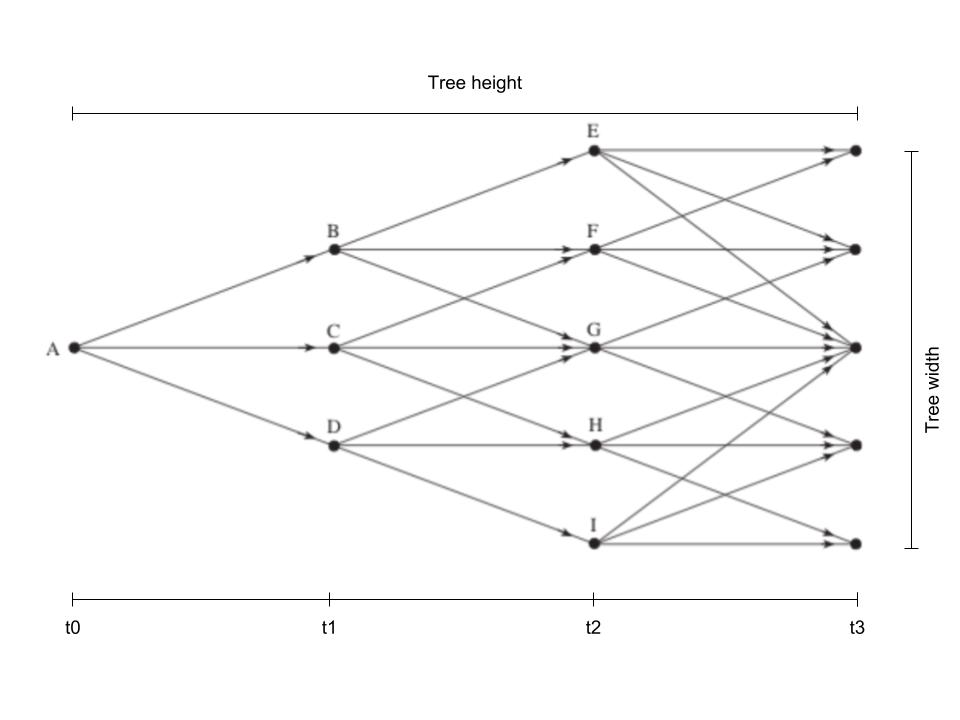
\includegraphics[width=0.8\textwidth]{img/treeconststage1wh.jpg}
	\caption{Example of the trinomial tree for $R^*$.}
	\source{Modified by the authors, based on Options, Futures and Other Derivatives\cite{ofod}[pg. 699].}
	\label{fig:treeconststage1}
\end{figure}

An important property of this tree include first of all that it is self-recombining, causing it to be symmetric. The probabilities on the lower part of the tree will be the negative of the probabilities on the upper part of the tree, e.g. probability that node A reaches node D is minus the probability of node A reaching node B. Furthermore, also due to symmetry, all unique probabilities can be stored in an array of size the width of the tree, because e.g. the probability of node A reaching node B is the same as the probability of node C reaching node F and so on. Probabilities are used both in stage 2 of the forward propagation, but also in the backward propagation, thus it is necessary to preserve them to the end, if they are to be stored. Last but not least, the way probabilities are calculated is different on $j_{min}$ or $j_{max}$, because of the difference in branching. 

\subsubsection*{Stage 2}
In this stage, the rates at each node in the tree at each time step are shifted up by an amount - $\alpha$, chosen so that the revised tree correctly prices discount bonds \cite[pg. 6]{uhwirt}. This is done by defining $Q_{i,j}$ as the present value of a security that pays off \$1 if node (i, j) is reached and 0 otherwise. The starting point is to set $Q_{0,0}=0$ and $\alpha_0$ to the interest rate at time $\triangle t$.$Q$s at the next time step are then calculated by using the generalized formula \cite[pg.705]{ofod}:  
\begin{equation}
\begin{gathered}
\begin{aligned}
Q_{m+1, j} = \sum_k Q_{m,k}q(k,j)exp[-(\alpha_m+k\triangle r)\triangle t]
\nonumber
\end{aligned}
\end{gathered}
\end{equation}
Supposing that we are starting on step $m$, to calculate the $Q$s on step $m+1$, we need to have the alpha on step $m$. Furthermore, once the $Q$s on step $m+1$ have been calculated, they are used to also find the alpha on $m+1$ later. This leads to conclude that alphas and $Q$s are interrelated on each time step. Alphas are calculated using the generalized formula \cite[pg.703]{ofod}:
\begin{equation}
\begin{gathered}
\begin{aligned}
\alpha_{m} = \dfrac{\sum_{j=-n_m}^{n_m} Q_{m,j}e^{-j\triangle r\triangle t} - \ln{P_{m + 1}}}{\triangle t}
\nonumber
\end{aligned}
\end{gathered}
\end{equation}
At the end of this stage, the new tree will have a similar shape to the one shown in fig. \ref{fig:treeconststage2}. 
\begin{figure}[H]
	\centering
	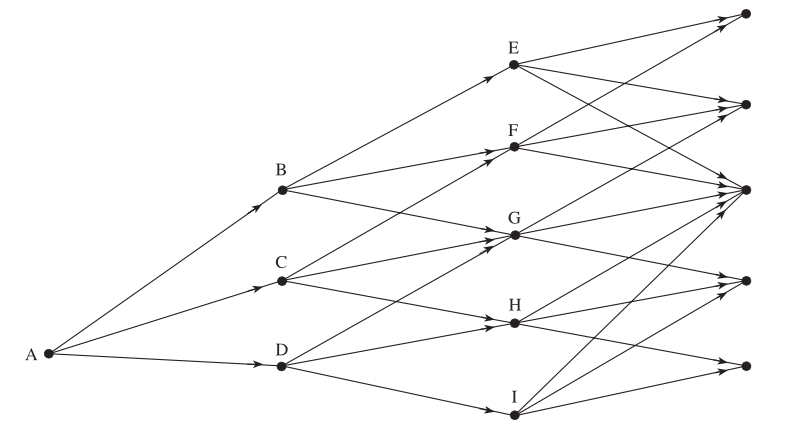
\includegraphics[width=0.8\textwidth]{img/treeconststage2.png}
	\caption{Example of the trinomial tree for $R$.}
	\source{Options, futures and other derivatives fig. 30.9 \cite[pg. 702]{ofod}}
	\label{fig:treeconststage2}
\end{figure}
An important observation here is that the only outcome of this tree that is used in the backward propagation is the array of alphas. $Q$s are in this case intermediary values, used to compute the alpha on each step and for this reason, the $Q$ values do not need to be stored any longer once all alphas have been computed. 
\subsection{Backward propagation}
The backward propagation starts with the previously constructed tree during the forward propagation step. At each time-step the option payoff is computed as the discounted value of the expected value at the next step \cite[pg. 6]{uhwirt}. From this it follows that the nodes at time step $i$ (e.g. the nodes without assigned letters in figures \ref{fig:treeconststage1} and \ref{fig:treeconststage2} above) are the starting point of the backward propagation. Their values are set to \$100 and are used to compute the previous set of nodes (at time step $i-1$). That is done by discounting these values from the actual strike price of the option, by using the array of alphas and the array of probabilities, both computed during the forward propagation. It is important to note that determining the final option value also depends on the type of option (whether it is a put or a call option). When the root of the tree is reached, the value at the root is the approximation of the option value and is the output of the algorithm. 

\section{Scatter vs. gather}
Both the forward and the backward propagation are composed of multiple aggregation operations, which is an overlay for multiple reads and writes of the data. There are two ways to perform the reads and writes of this data and it is important to choose the more performant one, as that may prevent data races in the following implementations. 

Taking the example from fig. \ref{fig:treeconststage1}, in order to compute the $Q$ value on node G in the forward propagation, values from nodes B, C and D have to be aggregated at node G. One approach to do that would be to calculate the values while located at each of the nodes B, C and D and write them to node G. This totals to a read and a write for each input node, or 3 reads and 3 writes. This operation is known as a scatter. On the other hand, the value of Q can also be computed when at node G, by reading the values of B, C and D and adding them in one place before writing the result on node G. This takes 3 reads and 1 write operations. This operation is known as gather. Since a write operations is more expensive, reducing the number of writes can have a crucial significance in parallel implementations, thus the second approach would always be preferable. In the backward propagation, the inverse intuition applies. E.g. the computation of the $call$ value at node C should be done while at node C, instead of while being at each of nodes F, G and H. While this should not produce any significant slowdown in the sequential implementation, or the one option per thread version, this thesis will focus on optimizing the writes in all of the implementations, by using gather. Note that using gather in the forward propagation can be non-trivial, as it requires various checks to be performed to avoid out-of-bounds array accesses. For this purpose, the sequential implementation will use scatter in the forward propagation, as it aims at simplicity and algorithm correctness and provides no challenges in terms of data races and hazards. Conversely, the rest of the implementations will only use gather operations.   